\documentclass{ctexart}
\usepackage{amsthm, amsmath, amssymb, amsfonts, esint, url, bytefield}
\usepackage{graphicx, float, xcolor, subcaption, enumitem, float}
\usepackage{geometry, hyperref, minted}

\geometry{
	a4paper,
	left=3.18cm,
	right=3.18cm,
	top=2.54cm,
	bottom=2.54cm
}

\setminted[c++]{
    frame=lines,
    linenos=true,
    breaklines=true
}


\title{\Large \textbf{HERMES}: s\textbf{H}allow dir\textbf{E}ctory st\textbf{R}ucture \textbf{M}any-fil\textbf{E} file\textbf{S}ystem \\ ——《存储技术基础》课程设计报告}

\author{计63\,\,陈晟祺\,\,2016010981 \\
计76\,\,刘晓义\,\,2017011426 \\
计72\,\,陈嘉杰\,\,2017011484 \\
计65\,\,高\hspace{1em}健\,\,2016011352}

\date{\today{}}

\begin{document}

\maketitle

\section{项目概述}

日常应用中,经常会出现目录层次较浅、文件很多而读取明显多于写入的情况;在开源镜像的建设中,这一情况尤为常见。常用的文件系统对于这一场景并没有进行很好的适配,导致目录枚举性能随文件数量增加而急剧下降。为了尝试缓解这一情况,我们设计了 HERMES,一个基于(多种可选的)开源键值存储引擎的 \texttt{FUSE} 文件系统,在文件数量较多的情况下也能进行较快的列举与读取。本项目在 \href{https://github.com/Harry-Chen/HERMES}{\textcolor{blue}{\texttt{GitHub}}} 以 MIT 协议开放源代码。

\section{项目背景}

开发本项目的动机来自一个真实的需求:\href{https://mirrors.tuna.tsinghua.edu.cn}{\textcolor{blue}{\emph{清华大学开源镜像站}}}为数百种开源软件提供二进制和源码的分发,通常提供 HTTP 与 HTTPS 协议供客户端下载,而提供 rsync 协议供下游镜像站同步。rsync 是一个增量的文件同步协议,工作流程大致如下(省略了一些算法细节):

\begin{enumerate}
    \item 客户端连接服务器,提供需要同步的目录和选项
    \item 服务器遍历指定目录,向客户端返回排序后的文件列表(包括元数据)
    \item 客户端根据元数据计算差异,得到需要同步的文件列表
    \item 客户端向服务器拉取需要的数据块(其中使用分块哈希进行增量)
\end{enumerate}

可以看到,在此过程中,客户端与服务器都需要对待同步的目录进行一次完全的递归遍历,并查询所有文件的元数据。大多数开源软件都有数十万个文件,因此每次遍历都会在服务器上产生较大的 IO 压力。为了解决这一问题,我们开发了 \href{https://github.com/tuna/rsync}{\textcolor{blue}{\texttt{rsync-huai}}},它将某个目录元数据预先遍历后放在内存中。这样只要文件不发生更改,之后的同步都不会再次触发文件夹的整体遍历,而只有文件读取开销。这有效地缓解了服务器的磁盘压力。

然而,这样的修改并不足够,一些软件源的结构带来了更大的麻烦。一个十分显著的例子为 \href{https://pypi.org/}{\textcolor{blue}{\texttt{PyPI}}},即 Python 语言官方的支持库发布站点。它的目录结构几乎是平坦的,其中存放有所有软件包的所有版本,只通过文件名进行区分。根据2019年6月6日的数据,PyPI 共有182500个项目,发布了1344057个版本,产生了1941223个文件,总容量约 5TB,是一个惊人的数字。当然,我们可以应用 \texttt{rsync-huai} 来缓解一些压力,但是事实上它本身的第一次遍历过程都会使得服务器磁盘响应延迟急剧增加,以至于同一台服务器上其他软件源几乎不响应请求。更糟糕的是,PyPI 更新速度相当快,因此如果使用这一解决方案,则每隔几个小时都需要重建整个内存索引,从而带来一段时间的服务降级。这会使得镜像站的用户体验质量下降,对于一个大型开源镜像站而言是不可接受的。

由于上述严重影响,我们只能关闭 PyPI 的 rsync 服务。但由于其体量巨大,官方的同步工具远没有 rsync 方便,并且上游连接性也有问题,如果我们不开放 rsync 服务,目前在中国大陆很难再对 PyPI 进行一次完全的初始同步。为了缓解这一问题,以能够更好地服务于国内的开源社区,这一问题需要得到缓解。

\section{项目实现}

\subsection{问题分析}

产生上述性能问题的主要原因是在大多数文件系统中,文件的遍历与检索都有较大的开销。如 \texttt{EXT} 文件系统中,每一个文件都有对应的 \texttt{inode},其中记录了元数据和文件数据对应的块编号等。为了查询一个 $n$ 层目录中文件的元数据,文件系统会进行以下的操作:

\begin{enumerate}
    \item 读取文件系统超级块,得到根目录的 inode 对应的块编号 $B_0$
    \item 读取 $B_1$ 得到根目录的 inode,找到第一级目录 inode 对应的块编号 $B_1$
    \item 重复上述操作,直到最后一级目录,此时找到了文件 inode 对应的块编号 $B_n$
    \item 读取 $B_n$,得到文件的元数据
\end{enumerate}

由于 inode 的存储并不连续,因此上述的块读取也都是零散的。而如果目录中文件有 $M$ 个,则需要将后两步重复 $M$ 次;并且文件数量越多,每次检索的读取次数越多(因为目录中文件列表无法在一个块中存下,需要更多的间接访问)。这样的非连续读取对于任何形式的磁盘与缓存机制都并不友好。虽然 \texttt{EXT4} 采取了 inode 连续预分配、使用带 Hash 的B树存储内容索引等措施,能够减少一部分非连续读写,并且操作系统对于文件的元数据访问有上层的缓存,但对于数百万个文件来说也只是杯水车薪。并且,镜像站由于管理等原因事实上使用了 \texttt{ZFS} 底层文件系统,其与带这些优化措施的 \texttt{EXT4} 相比,对于大量内容的目录遍历速度几乎慢了一个数量级。

有许多文件系统试图解决这一问题,对大量小文件的存储进行优化。如 \texttt{ReiserFS} 使用 B* 树存储文件元数据,加速寻址,降低文件检索的开销。Facebook 提出了 Heystack 用于保存其用户产生的海量小图片,淘宝也设计了 Tao File System 存储小文件。这些文件系统采取的措施都能够比较有效地解决小文件的存储与随机访问问题。不幸的是,它们都并没有对于文件列举这一特定需求进行针对性优化;并且,我们的应用场景并非只有小文件(很多文件达到数十 MB 量级)。因此,我们需要针对现实情况设计文件系统,来缓解这一问题。

一个简单而有效的想法是,我们需要对元数据存储的机制进行一些改进,如将其与文件分离存储,并将一个目录中的文件元数据尽量连续地存储。这样,对于一次完整的目录枚举,文件系统只需要定位到对应的目录元数据以后,连续地读取其子文件(夹)的元数据返回给系统即可。大大降低了对磁盘的读取压力。在写入时,则需要对于元数据进行更新,并进行预排序后写回。很明显,相较于普通文件系统,这可能降低写入操作的性能。但对于我们的应用场景而言,这是可接受的取舍,因为 PyPI 每次同步时不会删除任何历史文件,并且新增的文件也并不多。

进一步地,由于文件的目录层级并不深,我们也希望在检索时减小目录递归的开销。因此,我们选择使用键值存储的方式来保存元数据和文件内容。对于元数据,将文件/目录完整路径作为键,元数据作为值。对于文件内容,将其 ID 作为键,并将数据分块存储。具体细节可见下面的叙述。

此外,除了 rsync 服务之外,我们也需要对 PyPI 镜像提供普通的 HTTP(S) 服务。因此负载中也会有大量的文件直接请求,并且分布非常不均匀(如 \texttt{numpy} 等数十个热门包每天下载量为剩余所有包下载量之和)。因此,我们也需要探索合理的缓存机制,将热点文件缓存在内存中,以进一步减小对磁盘的压力。

\subsection{后端 API 设计}

目前比较流行的开源键值存储引擎有很多,我们选择了四个比较有代表性的:

\begin{description}
    \item[\href{https://github.com/google/leveldb}{\textcolor{blue}{\texttt{LevelDB}}}] Google 开发的高性能有序键值存储数据库。
    \item[\href{https://github.com/facebook/rocksdb}{\textcolor{blue}{\texttt{RocksDB}}}] Facebook 在 LevelDB 基础上改进的键值数据库,API 与其保持高度一致。
    \item[\href{https://www.oracle.com/database/technologies/related/berkeleydb.html}{\textcolor{blue}{\texttt{BerkeleyDB}}}] 最早由 UCB 开发的键值数据库,后被 Oracle 收购,支持大量语言与平台,支持部分特定的 SQL 语法。
    \item[\href{https://github.com/symisc/vedis}{\textcolor{blue}{\texttt{Vedis}}}] \texttt{Redis} 的嵌入式实现,支持 \texttt{Redis} 命令和 C 语言接口两种方式对数据进行操作,而且不需要经过网络。
\end{description}

程序使用一套公共的 API 操作键值引擎,并分别对每个后端适配这些 API。后端在 \texttt{CMake} 进行项目配置时即确定,并通过条件编译和模板静态分发等方式确定最终使用的代码。使用一个后端时无需编译或安装其他后端,也不会有额外的代码被编译或链接到最终的可执行程序中,并且切换后端不带来任何运行时开销。

具体地,为了使得前端代码可复用,我们要求每一个后端支持以下的公共 API:

\begin{minted}{c++}
// 获取新文件的 ID
uint64_t next_id();
// 写入文件元数据
write_result put_metadata(const std::string_view &path, const hermes::metadata &metadata);
// 读取文件元数据
std::optional<hermes::metadata> fetch_metadata(const std::string_view &path);
// 移除文件元数据
std::optional<hermes::metadata> remove_metadata(const std::string_view &path);
// 写入文件内容
write_result put_content(uint64_t id, size_t offset, const std::string_view &content);
// 获取文件内容
void fetch_content(uint64_t id, size_t offset, size_t len, char *buf);
// 移除文件内容
write_result remove_content(uint64_t id);
// 遍历目录内容
// 其中 F: (const std::string_view &path, const hermes::metadata &metadata) -> void 为对目录每个文件执行的访问器
template <typename F> inline void iterate_directory(const std::string_view &path, F accessor);
\end{minted}

考虑到 \texttt{FUSE} 的访问处理是并发的,以上实现都应该是线程安全的。

\subsection{后端实现}

后端的 API 本身已经比较明确地体现了我们元数据与文件内容分开的设计思路。我们在实现后端时,在这个思路上更进一步,将元数据和文件内容分别持久化在两个块设备上(或文件/目录,均可以由用户自行指定),实现了二者的完全分离。

在处理 \texttt{ls} 这类需要枚举目录内容的请求时(对应上述 \texttt{iterate\_directory} 接口),后端采取了两种不同的实现方案。除了 Vedis 的三种键值存储引擎都支持键的有序遍历。因此,这些后端可以直接以文件的完整路径作为 key 存储元数据;在需要列举目录内容时,从目录路径开始按顺序遍历引擎中的 key,直到找到目录中所有的内容为止。Vedis 则不支持键的有序遍历,后端必须在键值引擎中单独维护每个目录下的文件列表。

接下来,我们注意到,如果将整个文件的内容直接作为一个键值对的 value 存储起来,那么在修改文件内容时会产生很大的开销:取出全部文件内容,修改,然后再把全部内容插入回键值引擎。为了减少这种开销,我们在每个后端中都采用了分块策略存储文件内容:文件被划分为 4KB 大小的块,读写文件时只访问涉及到的那些分块。这样一来,读写的效率就大致和读写长度成正比,而不是和整个文件的长度成正比了。在此基础上,实现了稀疏文件比较高效的读写。

当然,因为采用了分块策略,所以我们还需要能够列举一个文件的所有分块,使得在删除文件时后端能把属于它的分块全部移除。这和上面所说的列举目录内容是十分相似的。对 LevelDB、RocksDB 和 BerkeleyDB 而言,我们把 \texttt{(id||offset)} 作为编号为 \texttt{id}、相对文件头偏移量为 \texttt{offset} 的分块的 key,就可以保证相邻的分块在数据库中也相邻存储,通过和遍历目录内容类似的方式遍历一个文件的所有分块,对文件的连续读写会转变为数据库的连续读写。作为实现细节的一环,这里需要把 \texttt{offset} 转换为大端序,保证它们的字节表示的顺序关系与数字的大小关系相同。Vedis 则仍然需要像上面一样,单独维护每个文件的分块列表,但无需在意端序问题。

符号链接可以直接在内部作为普通文件,将链接目标路径存入其内容中,这样对于符号链接的CURD操作就可以直接复用普通文件的CURD实现。

最后,四个键值引擎全部自带线程安全支持,无需编写额外的代码来确保多线程下的一致性。

\subsection{\texttt{FUSE} API 实现}

为了支持所需的文件操作,我们实现了以下的 \texttt{FUSE} API:

\begin{description}
    \item[\texttt{getattr}] 如果不是根,则调用 \texttt{fetch\_metadata},否则返回特定值。
    \item[\texttt{mkdir}] 调用 \texttt{put\_metadata} 写入指定的新元数据(ID为0,类型为目录)。
    \item[\texttt{unlink}] 调用 \texttt{remove\_metadata} 移除指定的元数据。
    \item[\texttt{symlink}] 创建符号链接,相当于普通文件的 \texttt{create + write}
    \item[\texttt{rmdir}] 直接转发到 \texttt{unlink} 进行处理。
    \item[\texttt{rename}] 将旧名称对应的元数据取出、移除后存为新的名称。
    \item[\texttt{chmod}] 修改元数据中用户ID对应字段并保存。
    \item[\texttt{chown}] 修改元数据组ID对应字段并保存。
    \item[\texttt{truncate}] 修改元数据尺寸对应字段,但不真正扩大大小,而是记录下待增大的大小。
    \item[\texttt{open}] 找到对应文件的元数据,将 ID 作为文件描述符返回。
    \item[\texttt{read}] 检查 \texttt{size} 尺寸后调用 \texttt{fetch\_content} 获取数据。
    \item[\texttt{write}] 检查 \texttt{size} 尺寸后调用 \texttt{put\_content} 写入数据。
    \item[\texttt{release}] 更新文件元数据(如修改时间和尺寸),并写回。
    \item[\texttt{readdir}] 调用 \texttt{iterate\_directory},将目录每一项都加入文件列表中。
    \item[\texttt{readlink}] 读取符号链接,相当于普通文件的 \texttt{open + read}
    \item[\texttt{init}] 初始化后端数据库引擎。
    \item[\texttt{destroy}] 释放后端数据库引擎。
    \item[\texttt{create}] 调用 \texttt{put\_metadata} 写入指定的新元数据(ID由 \texttt{next\_id} 获取,类型为文件)。
    \item[\texttt{utimens}] 修改元数据中访问时间、修改时间对应字段并保存。
\end{description}

具体的实现中涉及到错误处理等大量细节,需要考虑文件/目录不存在、权限不正确,读写大小越界等多种实际异常情况。由于篇幅原因,在此不加以详细描述。

当然,由于项目时间限制,我们也没有过多的兼容性需求,我们没有实现所有的 \texttt{FUSE} API;上述列出的API的实现大多也并不完整,或者与 POSIX/Linux 约定的有差异。例如 HERMES 并不支持硬链接、管道、设备等类型的文件,因为它们并不常用(在镜像站中实际也并没有被用到),而实现较为复杂(需要在几乎所有 API 进行特殊判断),支持这些类型并没有太大的意义。

\subsection{后端引擎细节}

\subsubsection{LevelDB}
LevelDB 提供的 API 包括:KV 的标准操作 Get、Put 和 Delete,用于查询、更新和删除键值对。这样根据上述描述的存储方式,可以简单的实现元数据的读、写以及删除,和文件内容块的读、写以及删除。

此外,LevelDB 还提供键空间的遍历,这样可以比较方便的实现列出目录,不需要单独存储每个目录的直接孩子。

这一遍历 API 存在的限制是:只能逐个遍历,以及 seek 跳转到第一个键不小于某个特定字符串的位置,为了保证我们在列出目录的时候能够在发现子目录的时候直接跳过子目录的内容,我们需要:

\begin{itemize}
    \item 子路径的内容的 metadata 紧跟着子路径的 metadata 存储
    \item 在 \texttt{iterate\_directory} 接口中,发现子路径时可以通过尽量少的数据库操作跳过这一子路径的内容
\end{itemize}

对于第一点要求,LevelDB 提供了自定义键之间全序关系关系的接口 (Comparator),只需要在比较路径的时候不是简单地根据 ASCII 字典序比较,而是把路径分隔符 / 作为字典的最小项再根据字典序比较,这样所有子路径在这种全序意义下会紧跟在父路径后面。

在此之上,跳过子路径的内容可以在一次 seek 内完成。例如如果在遍历 \texttt{/foo} 的时候发现了 \texttt{/foo/bar} 是一个目录,只需要 seek 到 \texttt{"/foo/bar/\textbackslash{}0xFF"},由于 0xFF 大于所有 POSIX 所允许的在路径中出现的 ASCII 字母,并且也大于所有 UTF-8 所表示的 Unicode Codepoint 中的第一个字节,这样可以保证直接跳过所有的 \texttt{/foo/bar} 路径内容。

此外,LevelDB 内置了缓存支持,可以建立自定大小的 LRU 缓存。在存储元数据和文件内容的两个 KV 数据库上都启用 128MB 的缓存可以保证大部分的元数据和最频繁读取的文件内容都在缓存中。

LevelDB 还内置了 CRC32 校验码计算,在文件系统挂载的时候进行自检。Valgrind 测试得到的数据显示 LevelDB 后端处理写入时在用户态中花费超过一半的时间在校验码的计算上。由于文件系统的目标用户会另行存储校验码,我们尝试重新编译了一个去掉了校验码计算的 LevelDB,但是测试中性能提升不明显。推测可能是因为 Valgrind 模拟器对于 CRC32 算法中密集的数值计算模拟性能不佳,导致给出了和真实硬件上运行相比不同的性能特征。为了方便分发,我们没有应用这个优化。

\subsubsection{RocksDB}

由于 RocksDB 与 LevelDB 的 C++ API 几乎是一致的,只在一些配置的修改上有些差别,因此两者几乎可共用同一份代码。我们使用预处理器完成了这一工作,根据选择的后端动态地对代码中的命名空间、变量、类型等进行重命名,并包含不同的头文件,以避免名称冲突与重定义等问题。经过这样的处理,LevelDB 的代码不需要太多修改就能够直接用于与 RocksDB 的适配。这样做避免了复制代码带来的行为不一致等潜在隐患。

\subsubsection{BerkeleyDB}

BerkeleyDB 是我们所用到的四个后端中最古老的一个(1990年代),它支持 Hash BTree Queue 和 Recno 等多种存储方法,功能完整,使用广泛。我们仅使用了 BerkeleyDB 的 BTree 存储结构;也因为是 BTree,性能指标和文件系统 \texttt{EXT4} 比较相似:相比而言写性能比较高、读性能比较低。我们对其进行一些性能优化:增大缓存,这显著地减少了缓存缺失的比例,使得读取性能有了显著的提升;添加多线程支持,顺序读写性能会有略微的降低,但随机读写的性能有了不错的提升,这和 CPU 缓存的特征是比较一致的。

代码在编写的时候,尽量减少了不必要的内存分配和释放:从数据库读取的时候,直接把目标地址传给 BerkeleyDB 以减少一次额外的复制,也采用了栈空间作为读取的缓存来代替堆的分配。

如果按照日常使用的读写的比例的话,BerkeleyDB是比较适合作为文件系统后端的。

\subsubsection{Vedis}

Vedis 的特点是 Redis 命令的嵌入式 C 实现。但是,我们并未充分利用这一特性,而是使用了裸的键值引擎访问接口。这有三个原因:首先,运行时按照 C 的格式化字符串风格解析命令会带来额外的数据复制开销;其次,使用 Redis 命令意味着插入的数据必须是可见字符串,这对于需要存储字节流信息的文件系统来说比较不能接受;最后,Vedis 并不是支持全部的 Redis 命令,一些比较关键的命令没有实现。

另外,如同上面所说,Vedis 不支持键的有序遍历,这是比较致命的;通过裸的键值引擎接口难以解决这个问题,我们退而求其次选择使用 Vedis 提供的 Redis 集合指令来存取每个目录的内容。文件的分块列表也采用同样的手段处理。由于有字符串复制和指令解析的操作,这一步引入了较大的开销。

整体上来看,Vedis 为了维护目录和文件的内容存储了额外的键值对,其数量正比于(传统)文件系统中 inode 的数量,维护它们的代价也相对较大。在后续的测试中我们可以看到,这比较严重地拉低了 Vedis 后端的读写性能。实践证明,作为一个原生不支持键的有序遍历的引擎,Vedis 是不太适合作为文件系统后端的。

\subsection{编译运行}

可参考代码目录中的 \texttt{README.md} 以获得关于编译和运行 HERMES 的指示。

\section{项目测试}

\subsection{测试环境}

本项目测试的机器配置与系统环境为:

\begin{description}
    \item[CPU] Intel Xeon E5-2670 v3
    \item[RAM] DDR4 2133 16GB * 8
    \item[SSD] Intel SSDPEKKW010T7 1TB
    \item[Software] Arch Linux (2019/6/8 latest), FUSE 2.9.9 (Use 2.6 API)
\end{description}

所用到的测试脚本位于代码目录的 \texttt{tests} 文件夹中,可按照相应的指示运行。

\subsection{正确性测试}

正确性是文件系统的根基,但我们的实现不可避免地会存在问题。为了保证实现的正确性,我们编写了自动化测试脚本,对于每个后端,分别执行随机读写、文件校验和比对、反复重新挂载、创建与删除大量文件等基本的正确性测试,一方面保证文件的存储正确,另一方面也测试实现的鲁棒性。在保证实现正确且安全的情况下,谈论性能才是有意义的。

\subsection{性能测试}

为了检验实现的效率,我们对于每一个后端都进行了一系列的性能测试,并以 \texttt{EXT4} 文件系统作为对照。测试内容包括不同块大小(包括1KB、4KB、16KB)的连续/随机文件读写带宽,以及一定数量的(1000到1000000)文件创建/枚举时间。我们将使用 \texttt{fio} 工具与自己编写的测试脚本综合进行测试,每项将进行多次测试,取\textbf{最大值}。

\subsubsection{文件读写性能}

表\ref{tab:seq-read}, \ref{tab:seq-write}, \ref{tab:rand-read}, \ref{tab:rand-write}分别为连续/随机文件读/写的性能测试结果。需要注意下列所有数据的词头进制都为 1024。我们将这些表格中的数据使用对数坐标绘制为图\ref{fig:seq-read}, \ref{fig:seq-write}, \ref{fig:rand-read}, \ref{fig:rand-write}中的柱形,可以更直观地看到各个后端的性能差异。

先考虑读取,可以看到无论每次读取的大小,HERMES 基于 LevelDB 和 RocksDB 的实现都有远高于 \texttt{EXT4} 文件系统的性能(前者更优,最高可达到 \texttt{EXT4} 十倍以上),而访问是否有顺序性几乎完全不影响任何指标。这是由于它们的内部实现都比较类似,有较大的 LRU 缓存,并且专门为此类场景进行优化,因此有相当大的优势。而 BerkeleyDB 虽然没有使用大缓存,在所有测例上的性能也高于 \texttt{EXT4}(最高也有三倍左右)。这说明我们设计的存储方式的确具有一定的优越性。此外,Vedis 的表现十分平庸,无法与其他的后端相比。

在写入上,表现与读取恰恰相反。当单次访问较大的块时,\texttt{EXT4} 的性能总是高于 HERMES。在 HERMES 的后端中比较, BerkeleyDB 与 RocksDB 没有显著的差别,都随着单次访问大小增加有较大的提升(前者稍显优势);LevelDB 与 Vedis 表现得不尽人意,前者随机写入带宽较低,后者无论是否顺序都维持在较低的水平。这是预期之中的表现:由于键值存储的特性,HERMES 进行写入时,总是需要更新整个文件;而即使采用了数据分块的方式缓解这一问题,复杂度依旧比较高。因此,相对于 \texttt{EXT4} 优化后几乎与写入次数呈线性关系的时间开销,HERMES 在访问块较大时 自然无法获胜。虽然如此,各项数据也都在可接受的范围内。考虑到真正应用场景中几乎都是单次连续写入(创建新文件),目前的吞吐量(约 80 到 100MBps 量级)不会成为整个系统的瓶颈。

为了与真正的应用场景匹配,我们使用了另外的评测环境,将 \texttt{EXT4} 替换为(镜像站实际使用的) \texttt{ZFS} 重复了上述测试。由于篇幅原因,在此不提供详细数据(包含在提交的文件中)。测试结果表明,\texttt{ZFS} 或许对顺序读写进行了专门的优化:读取最快能达到 LevelDB 的吞吐量的 $80\%$ 左右,而写入吞吐量可达到最快的 BerkeleyDB 的五倍多,HERMES 的性能优势被削弱了。但是在随机读写方面,\texttt{ZFS} 表现欠佳:读取与 BerkeleyDB 接近,但只有 LevelDB 的三分之一左右;而写入性能几乎无法超过 HERMES,只在单次访问 16K 时能够超过 LevelDB,只有最快的 RocksDB 的六分之一。这意味着 HERMES 在读或随机访问占优的应用场景中,相比 \texttt{ZFS} 有较大的(吞吐量)性能优势。

\begin{table}[htbp]
\centering
\caption{顺序读取性能(单位:MBps)}
\label{tab:seq-read}
\begin{tabular}{cccccc}
\hline
单次访问大小 & EXT4 & LevelDB & RocksDB & BerkeleyDB & Vedis \\ \hline
1KB     & 100  & 248     & 292     & 112        & 31.1  \\
4KB     & 399  & 990     & 1064    & 436        & 64.1  \\
16KB    & 380  & 3907    & 3749    & 996        & 82.6  \\ \hline
\end{tabular}
\end{table}

\begin{figure}[htbp]
\centering
\caption{顺序读取性能对比}
\label{fig:seq-read}
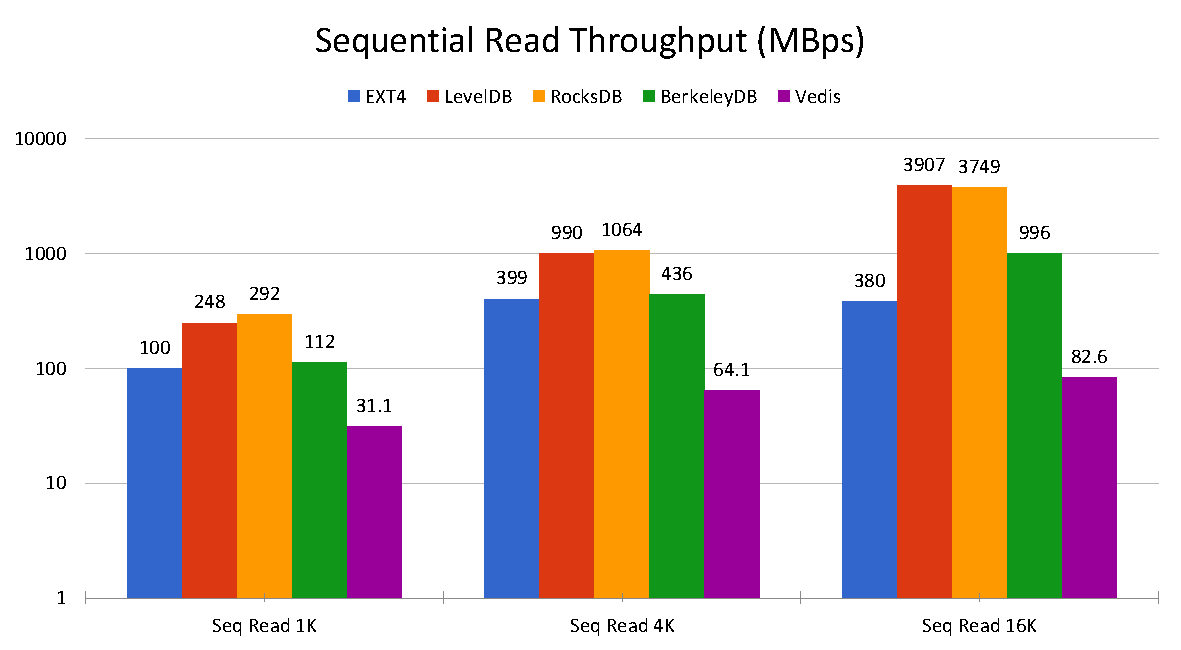
\includegraphics[page=1,width=\textwidth]{HERMES_perf_plot.pdf}
\end{figure}


\begin{table}[htbp]
\centering
\caption{顺序写入性能(单位:MBps)}
\label{tab:seq-write}
\begin{tabular}{cccccc}
\hline
单次访问大小 & EXT4 & LevelDB & RocksDB & BerkeleyDB & Vedis \\ \hline
1KB     & 50.1 & 20.7    & 18.1    & 18.8       & 19.2  \\
4KB     & 406  & 80.2    & 76.6    & 59.5       & 26.7  \\
16KB    & 434  & 112     & 120     & 130        & 40.5  \\ \hline
\end{tabular}
\end{table}

\begin{figure}[htbp]
\centering
\caption{顺序写入性能对比}
\label{fig:seq-write}
\includegraphics[page=2,width=\textwidth]{HERMES_perf_plot.pdf}
\end{figure}


\begin{table}[htbp]
\centering
\caption{随机读取性能(单位:MBps)}
\label{tab:rand-read}
\begin{tabular}{cccccc}
\hline
单次访问大小 & EXT4 & LevelDB & RocksDB & BerkeleyDB & Vedis \\ \hline
1KB     & 99.8 & 227     & 266     & 136        & 28.1  \\
4KB     & 399  & 892     & 1039    & 557        & 59.2  \\
16KB    & 279  & 3824    & 3097    & 928        & 74.8  \\ \hline
\end{tabular}
\end{table}

\begin{figure}[htbp]
\centering
\caption{随机读取性能对比}
\label{fig:rand-read}
\includegraphics[page=3,width=\textwidth]{HERMES_perf_plot.pdf}
\end{figure}


\begin{table}[htbp]
\centering
\caption{随机写入性能(单位:MBps)}
\label{tab:rand-write}
\begin{tabular}{cccccc}
\hline
单次访问大小 & EXT4  & LevelDB & RocksDB & BerkeleyDB & Vedis \\ \hline
1KB     & 8.119 & 9.93    & 13.2    & 16.1       & 16    \\
4KB     & 384   & 22.3    & 81.4    & 66.3       & 29.2  \\
16KB    & 425   & 22.8    & 118     & 122        & 34.1  \\ \hline
\end{tabular}
\end{table}

\begin{figure}[htbp]
\centering
\caption{随机写入性能对比}
\label{fig:rand-write}
\includegraphics[page=4,width=\textwidth]{HERMES_perf_plot.pdf}
\end{figure}

\subsubsection{元数据读写性能}

针对上面提出的问题,我们测试了修改元数据的性能,即先创建若干个文件并计时,再使用 \texttt{ls} 命令枚举这些文件及其属性(将输出丢弃)并计时。表 \ref{tab:file-create}, \ref{tab:file-enumerate} 为测试得到的数据,图 \ref{fig:file-create}, \ref{fig:file-enumerate} 为根据表中数据绘制的对比柱状图。

可以看到,在文件创建这一指标上,HERMES 几乎总是慢于 \texttt{EXT4} 文件系统,耗时约为6到7倍。考虑到我们实现的存储方式与 \texttt{EXT4} 在新建文件时都有 $\mathcal{O}(n \log n)$ 的时间复杂度开销,但 \texttt{EXT4} 相对进行了较多的优化(如预分配),因此这一结果是预期中的。也可以看出,对于每一个后端,随着文件数量增多,时间增长尚且呈现线性趋势(因为在文件系统合理文件数量范围内 $\log n$ 总可以看成一个较大的常数)。BerkeleyDB 由于在小块随机写入上有性能优势(从读写性能测试中能够发现),所以耗时也相对较短。


%在文件枚举上,\texttt{EXT4} 依旧有一定的优势(1000000 个文件时约比最快的 HERMES 后端快 $60\%$),不过这并不意味着 HERMES 没有达到它的目标。事实上,\texttt{ls} 进行文件枚举共分两步:首先调用 \texttt{readdir} 获取目录中每个文件的简要信息;而后如果需要(如带有 \texttt{-l} 参数),再调用 \texttt{stat} 获取每个文件的详细元数据。程序可以在调用 \texttt{readdir} 时告知系统对文件元数据进行预取,这样可以节省大量的重复的元数据读取,也可以在不需要的时候不进行过多读取,\texttt{EXT4} 会很好地利用这一特性。而由于我们使用的 \texttt{FUSE} 库的具体实现在调用相关函数时并不会携带这一信息,HERMES 总是会在 \texttt{readdir} 阶段返回所有的元数据,而在 \texttt{stat} 阶段进行重复的读取,从而导致性能下降。此外,FUSE 强迫使用它提供的回调进行目录信息的填充。这即是说,对于目录下的每一个文件和子目录,都需要进行一次系统调用拷贝元数据,这是 \texttt{EXT4} 所没有的额外开销。并且 \texttt{FUSE} 本身工作在用户态,在读写与交互底层文件时也因为系统调用而产生较大的开销。

在文件枚举上,\texttt{EXT4} 依旧有一定的优势(1000000 个文件时约比最快的 HERMES 后端快 $60\%$),不过这并不意味着 HERMES 没有达到它的目标。Linux 内枚举目录内容的工作方式是创建一个接受目录内容的缓冲区,调用 \texttt{syscall getdents}。FUSE2 在内核模块和用户态程序之间传递目录内容的方式是一个链表,之后 FUSE2 会将链表内容逐个复制进缓冲区内。相比之下,对于工作在内核态的 \texttt{EXT4} 驱动可以直接写入 \texttt{syscall getdents} 调用者提供的缓冲区,相比之下在驱动层减少了一次复制。 

此外,我们的目录枚举可以同时返回所有内容的元数据,但是 FUSE2 没有提供这样的接口。升级到 FUSE3 之后虽然提供了在枚举的同时返回元数据的接口,但是此时 FUSE 内核模块和用户态程序之间的数据传递不再使用链表,而是使用线性数组。FUSE 在内核模块中限制了每次和用户态程序的通信数据量最多只有一个页的大小 (\texttt{PAGE\_SIZE}),在大多数内核中这个常数都是 4KB,考虑元数据的大小,我们大约每次都只能返回 25 个左右的目录内容项。此时 FUSE3 也不会在内核模块中检查是否 \texttt{syscall getdents} 调用方的缓存已满,而是直接返回。因此无论调用方传递了多大的缓存,每次最多只能得到 25 个左右的目录项,列出大目录的时候需要反复调用 \texttt{syscall getdents},每次调用会涉及两次内核和用户态的通信,这带来的性能影响是巨大的。

所以在升级到了 FUSE3 之后,虽然在使用 \texttt{ls -fl} 带元数据地列出目录时可以获得和不带元数据完全一致的性能,但是每次列出 1M 目录项需要的时间上升至原来的4倍左右,而且需要修改后端的实现,以满足列出目录的初始偏移量,带来更高的实现复杂度,否则列出目录由于中途会被打断,时间复杂度会上升到 $\mathcal{O}(n^2)$ 的水平。

综合上述原因,在如此多的不利条件下,我们的目录枚举速度依旧能与 \texttt{EXT4} 相近,并且产生的 IO 压力更小(使用 \texttt{iotop} 工具在 \texttt{ls} 运行时观察底层块设备的利用率可知),说明 HERMES 拥有较大的优化空间。如将其编写为内核模块,则能够省去大量不必要的开销,得到较大的性能提升。

我们同样也在 \texttt{ZFS} 上进行了这一测试。在该平台上,\texttt{ZFS} 的文件创建速度并没有显著优势,与 BerkeleyDB 为后端时较接近。在文件枚举上,\texttt{ZFS} 也快于 HERMES(与 \texttt{EXT4} 表现类似)。考虑到上述的原因,可以认为 HERMES 相较于 \texttt{ZFS},在元数据修改方面也有较大的优化潜力。


\begin{table}[htbp]
\centering
\caption{文件创建耗时(单位:毫秒)}
\label{tab:file-create}
\begin{tabular}{cccccc}
\hline
文件数量    & EXT4  & LevelDB & RocksDB & BerkeleyDB & Vedis  \\ \hline
1000    & 22    & 76      & 80      & 54         & 95     \\
10000   & 144   & 721     & 795     & 370        & 938    \\
100000  & 1089  & 7735    & 8403    & 3482       & 9547   \\
1000000 & 14755 & 88589   & 109558  & 35151      & 132577 \\ \hline
\end{tabular}
\end{table}

\begin{figure}[htbp]
\centering
\caption{文件创建耗时对比}
\label{fig:file-create}
\includegraphics[page=5,width=\textwidth]{HERMES_perf_plot.pdf}
\end{figure}


\begin{table}[htbp]
\centering
\caption{文件枚举耗时(单位:毫秒)}
\label{tab:file-enumerate}
\begin{tabular}{cccccc}
\hline
文件数量    & EXT4 & LevelDB & RocksDB & BerkeleyDB & Vedis \\ \hline
1000    & 3    & 3       & 3       & 3          & 7     \\
10000   & 14   & 15      & 17      & 13         & 45    \\
100000  & 56   & 106     & 136     & 94         & 387   \\
1000000 & 537  & 918     & 967     & 851        & 3929  \\ \hline
\end{tabular}
\end{table}

\begin{figure}[htbp]
\centering
\caption{文件枚举耗时对比}
\label{fig:file-enumerate}
\includegraphics[page=6,width=\textwidth]{HERMES_perf_plot.pdf}
\end{figure}

\subsection{测试结论}

通过上述的测试,我们可以认为 HERMES 的性能达到了我们的设计预期,即成功地对目录枚举进行了加速,并对读取热点进行了缓存以得到极大的性能提升;此外,在写入上,HERMES 相对于现有文件系统的性能损失也可以接受,不会在我们预设的PyPI镜像这一应用环境中产生瓶颈。

关于后端的选择,可以看到除了 Vedis 表现不佳外,其余三个键值存储引擎各有所长。读与写性能是很难兼得的,因此三个引擎呈现了比较鲜明的特征:LevelDB 长于读取,RocksDB 比较均衡,而 BerkeleyDB 写入性能强劲。考虑到三者的发展与现状,以及实际的应用场景,我们认为 RocksDB 是最适合于 HERMES 的后端:它既没有 BerkeleyDB 的历史包袱,也在 LevelDB 极强读取性能的基础上进一步优化了写入性能,从而能在读占优的场景中取得最好的表现。

\section{总结}

本项目中,我们实现了 HERMES,一个基于键值存储的 FUSE 文件系统。事实上,如果在 GitHub 上检索,并不缺乏类似的工作,如 \href{https://github.com/qznc/kvfs}{\textcolor{blue}{\texttt{kvfs}}} 等。但与它们相比,HERMES 得完成度更高:支持多个后端切换、性能参数经过精细调节、在多个测例上能稳定胜过现有文件系统;并且,HERMES 是为了一个真实存在的问题而设计的,它的确也成功地缓解了这一问题。因此,我认为 HERMES 达到了我们最初的目标。

必须要承认,作为课程作业,项目的完成比较仓促。无论是性能上,还是实现的功能上,我们的实现还有巨大的改进空间:一定还有我们没有发现的种种问题存在,也一定有大量的边角情况没有得到处理。所以,HERMES 离一个成熟的文件系统还差很远,离真正被部署到生产服务器上也还有很长的一段路要走。

重要的是,在HERMES开发过程中,我们也了解了很多“背后的世界”:比如每一个简单文件操作会变成多少底层调用,Linux 内核为了提高IO性能又做了什么。我们会使用工具一遍又一遍调整参数、测试性能,直到代码中隐藏的问题被解决,得到我们预期的结果;也会花一晚上追踪 FUSE 的源码,找到性能瓶颈所在(并放弃无谓的优化);甚至还会为了代码的优雅学习现代C++。与其他组的成果相比,HERMES 可能并不够有趣,因为它能做的并不超出任何现有文件系统的能力范围,甚至实现上更不完整,也没有任何能够吸引眼球的成果可供展示。但我们相信,完成这一项目给我们带来的收获要远胜于那些 fancy 的展示效果:让我们知道文件系统究竟如何工作,性能又被什么影响。因此,HERMES 的开发对我们而言有着重要的意义。

此外,在 HERMES 的开发过程中,于纪平同学提供了大量技术上的指导(主要关于C++特性),在此特别向他表示感谢。

\end{document}
